\section{Inverse Gamma Distribution}

\subsection{Standard Inverse Gamma Distribution}

The pdf of the inverse gamma is 

\begin{equation}
	f(x, \alpha, \lambda) = \frac{\lambda^{\alpha}}{\Gamma(\alpha)} x^{-\alpha-1} \exp(-\frac{\lambda}{x})
	\label{eq:pdf_inverse_gamma}
\end{equation}

where $\Gamma$ is the Gamma function. This can be rewritten as

\begin{equation}
	f(x, \alpha, \lambda) = \exp \left[(-\alpha-1)\log(x) - \lambda/x + \alpha \log(\lambda) -\log\Gamma(\alpha)\right]
	\label{eq:exp_inverse_gamma}
\end{equation}

where $T=(\log(x), x), \eta= (-\alpha-1, -\lambda)$ and $A(\alpha,\lambda) = \log\Gamma(\alpha) - \alpha\log\lambda$.

\subsubsection{Laplace Approximation of the standard inverse gamma distribution}

\begin{align*}
\text{log-pdf: } &(-\alpha-1)\log(x) - \lambda/x + \alpha \log(\lambda) -\log\Gamma(\alpha) \\
\text{1st derivative: }&  \frac{-\alpha-1}{x} + \frac{\lambda}{x^2}\\
\text{mode: }& \frac{-\alpha-1}{x} + \frac{\lambda}{x^2} = 0 \Leftrightarrow x = \frac{\lambda}{a+1}\\
\text{2nd derivative: }&  \frac{\alpha+1}{x^2} - 2\frac{\lambda}{x^3}\\
\text{insert mode: }& \frac{\alpha+1}{\frac{\lambda}{a+1}^2} - 2\frac{\lambda}{\frac{\lambda}{a+1}^3} = -\frac{(\alpha +1)^3}{\lambda^2} \\
\text{invert and times -1: }&\sigma^2 = \frac{\lambda^2}{(\alpha +1)^3}
\end{align*}

\subsection{Sqrt-Transform of the inverse Gamma distribution}

TODO: Double-Check this whole sqrt business.

\subsubsection{Laplace Approximation of the sqrt-transformed Inverse Gamma Distribution}

\begin{align*}
\text{log-pdf: } &-2\alpha\log(x) - \frac{\lambda}{x^2} + \alpha \log \lambda - \log\Lambda(\alpha) \\
\text{1st derivative: }& -\frac{2\alpha}{x^2} + 2\frac{\lambda}{x^3} \\
\text{mode: }&  x = \sqrt{\frac{\lambda}{\alpha}}\\
\text{2nd derivative: }&  \frac{2\alpha}{x^2} - 6\frac{\lambda}{x^4}\\
\text{insert mode: }&  -4\frac{\alpha^2}{\lambda}\\
\text{invert and times -1: }&\sigma^2 = \frac{\lambda}{4 \alpha^2}
\end{align*}

\subsubsection{The Bridge for the sqrt-transformed Inverse Gamma Distribution}

\begin{align}
\mu &= \sqrt\frac{\lambda}{\alpha} \\
\sigma^2 &= \frac{\lambda}{4\alpha^2} \\
\alpha &= \frac{\mu^2}{4\sigma^2}\\
\lambda &= \frac{\mu^4}{4\sigma^2}\\
\end{align}

\subsection{Log-Transform of the inverse Gamma distribution}

We choose $g(x) = \log(x)$, and thereby $g^{-1}(x) = \exp(x)$. It follows that the new pdf is 

\begin{equation}
	f_t(x, \alpha, \lambda) = \frac{\lambda^{\alpha}}{\Gamma(\alpha)} \exp(x)^{-\alpha} \exp(-\lambda/\exp(x))
	\label{eq:inv_gamma_trans_pdf}
\end{equation}

which can be written as 

\begin{equation}
	f_t(x, \alpha, \lambda) = \exp \left[-\alpha x - \frac{\lambda}{\exp(x)} + \alpha \log \lambda - \log\Lambda(\alpha)\right]
\end{equation}

with $T=(x, 1/\exp(x)), \eta(-\alpha, \lambda)$ and $A(\alpha, \lambda) = \log\Gamma(\alpha) - \alpha \log \lambda$.

\subsubsection{Laplace Approximation of the log-transformed Inverse Gamma Distribution}


\begin{align*}
\text{log-pdf: } &-\alpha x - \frac{\lambda}{\exp(x)} + \alpha \log \lambda - \log\Lambda(\alpha) \\
\text{1st derivative: }&  -\alpha + \frac{\lambda}{\exp(x)}\\
\text{mode: }&  -\alpha + \frac{\lambda}{\exp(x)} = 0 \Leftrightarrow x = \log(\lambda/\alpha)\\
\text{2nd derivative: }&  -\frac{\lambda}{\exp(x)}\\
\text{insert mode: }&  -\frac{\lambda}{\exp(\log(\lambda/\alpha))} = -\alpha\\
\text{invert and times -1: }&\sigma^2 = \frac{1}{\alpha}
\end{align*}

\subsubsection{The Bridge for the log-transformed Inverse Gamma Distribution}

\begin{align}
	\mu &= \log\left(\frac{\lambda}{\alpha}\right) \\
	\sigma^2 &= \frac{1}{\alpha} \\
	\alpha &= \frac{1}{\sigma^2}\\
	\lambda &= \frac{\exp(\mu)}{\sigma^2}\\
\end{align}

\begin{figure}
	\centering
	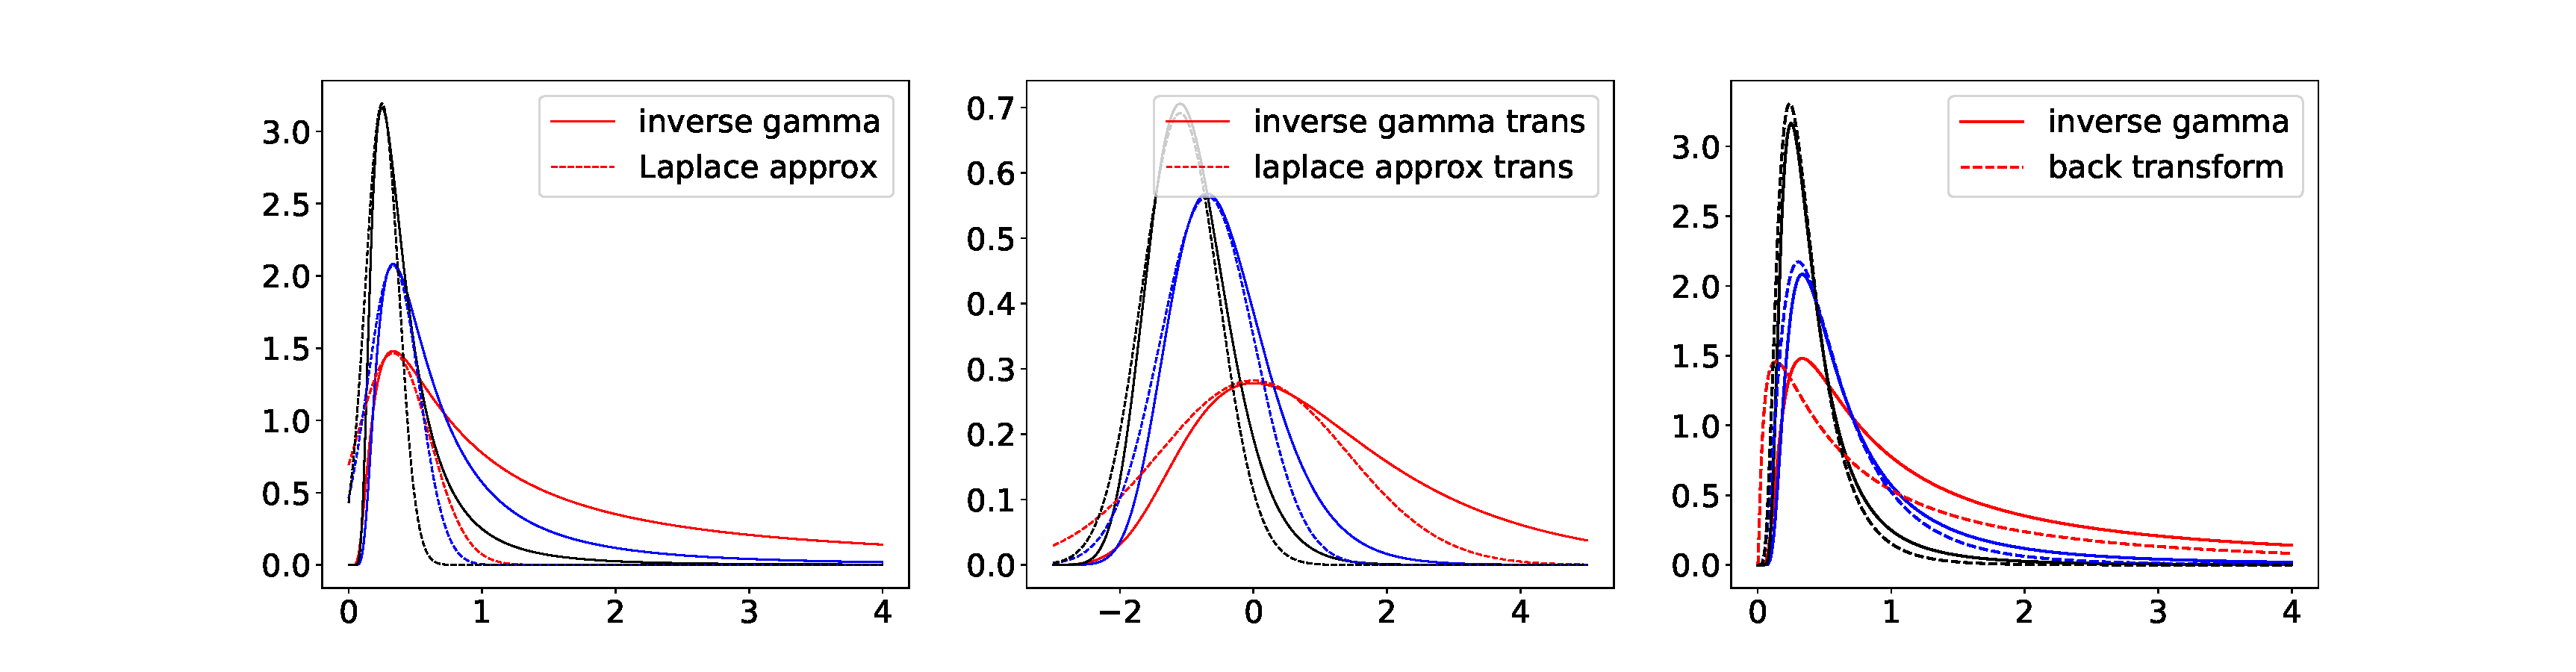
\includegraphics[width=\textwidth]{figures/inverse_gamma_playground.pdf}
	\caption{inverse gamma comparison}
	\label{fig:inverse_gamma_comparison}
\end{figure}